\section{Discussion} \label{sec:Discussion}
\subsection{Comparison to observations}
\textit{Gaia}-Enceladus \cite{Enceladus....Helmi...2018}
sagitarius modellierung single orbit Beispiel
-> zeigen dass kein single orbit ist (literatursuche)

\begin{figure}[htbp]
    \centering
    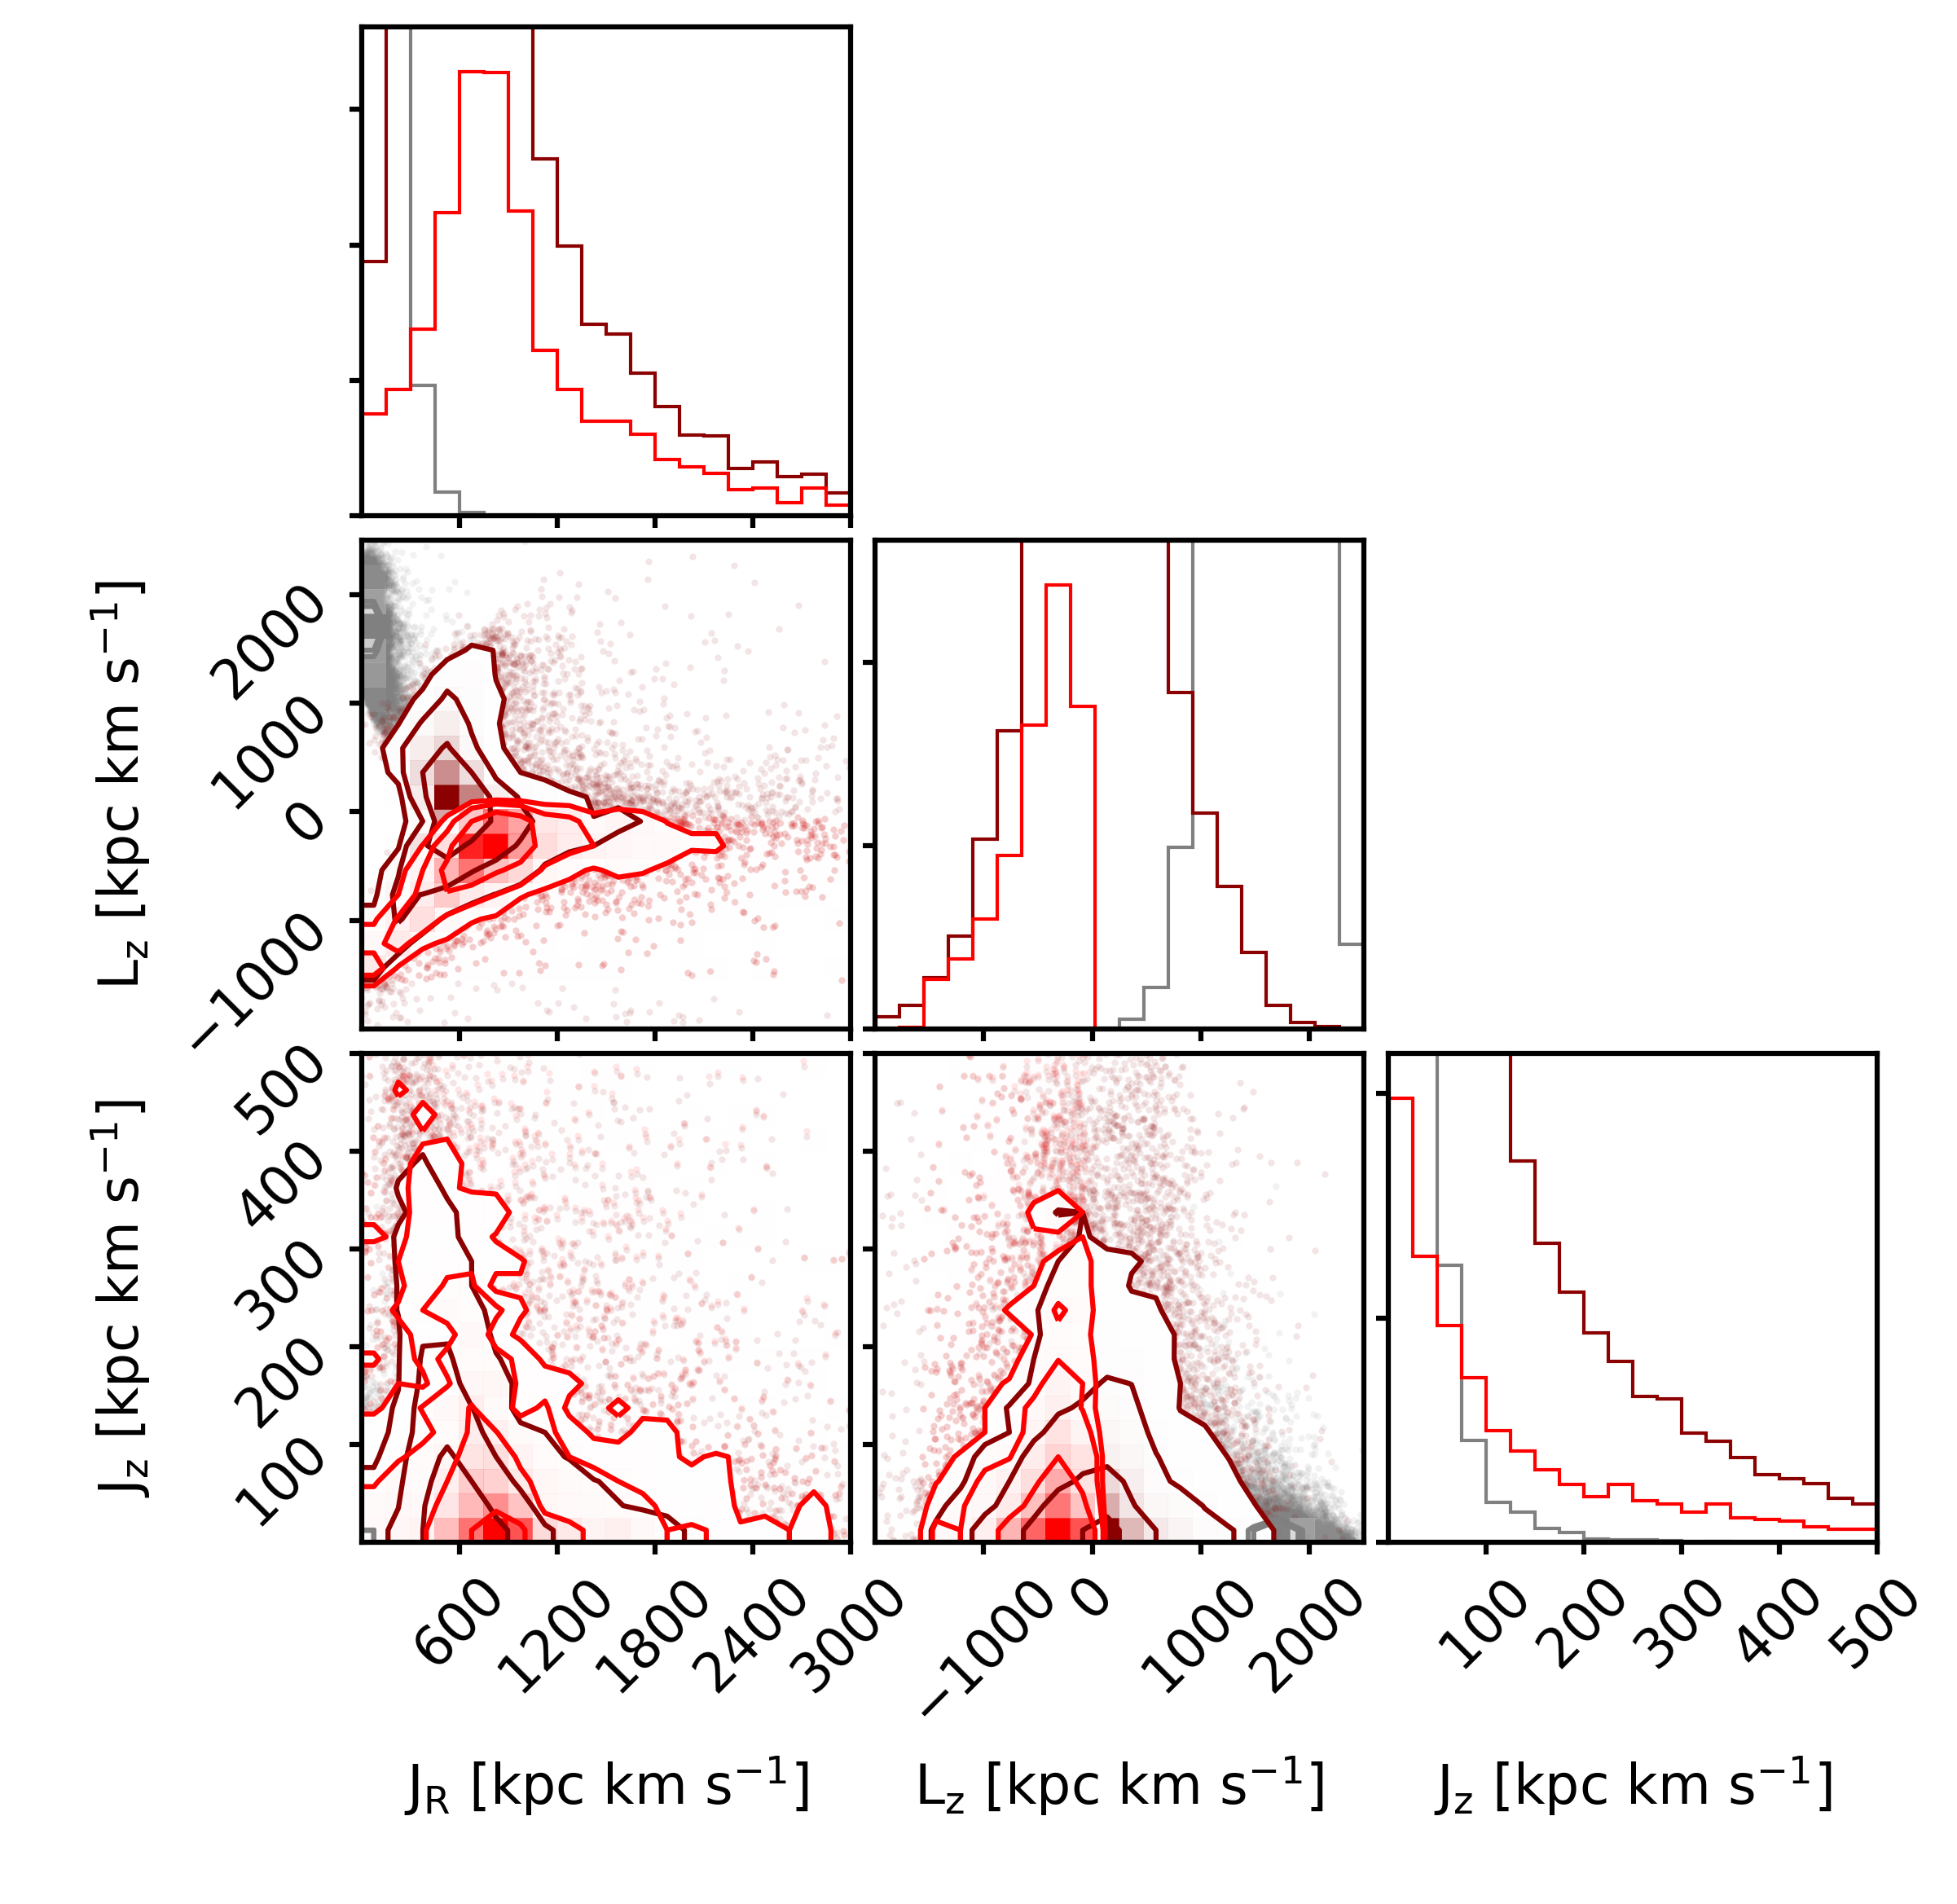
\includegraphics[width=1.0\textwidth]{plots/Discussion/Gaia_all_actions_MW14_talk3.png}
    \caption{\textit{Gaia} Enceladus in action space in the MW14Potential.}
    \label{fig:act_both_merg_best_pot}
\end{figure}

\subsection{Comparison to literature}
richtige verteilunggsfunktion fuer accreted teilchen zu bestimmen 

\subsection{Caveats}

\subsection{Future Work}